\chapter{Concepts théoriques de base}
\label{chap:preliminaries}

\section{Introduction}

Ce chapitre présente les concepts nécessaires à l'étude de la formation de formes décentralisée : robotique en essaim, inspirations biologiques, consensus, flocking, représentation géométrique de la cible et passage de messages sur graphe. Il précise les propriétés de localité, de connectivité et de partage des paramètres qui serviront à analyser les méthodes du chapitre~\ref{chap:etat-art}. Ces notions fournissent un cadre théorique et un vocabulaire commun ; elles ne constituent pas une validation empirique du contrôleur. Les exemples relatifs au projet décrivent les choix du prototype historique ; les résultats correspondants sont distingués de la validation expérimentale encore attendue pour l'implémentation actuelle.

\section{Robotique en essaim et contrôle décentralisé}

La robotique en essaim s'intéresse à la coordination d'agents nombreux, homogènes ou faiblement hétérogènes, qui accomplissent collectivement une tâche sans dépendre d'un superviseur unique. La revue de Brambilla et al. souligne que cette approche associe généralement simplicité individuelle, redondance et interactions locales \cite{brambilla2013}. L'objectif n'est pas seulement de répartir une tâche entre plusieurs robots : il est de concevoir des règles locales dont l'effet collectif reste utile lorsque la taille du groupe, la topologie de communication ou la disponibilité des agents évoluent.

Les modèles comportementaux ont fourni des exemples fondateurs de cette idée. Le modèle de Reynolds repose sur trois mécanismes simples --- séparation, alignement et cohésion --- qui génèrent des déplacements collectifs crédibles sans plan global explicite \cite{reynolds1987}. Dans un cadre de contrôle multi-agent, Olfati-Saber formalise des lois de flocking qui combinent cohésion, évitement de collision et maintien de la connectivité à travers un graphe d'interactions \cite{olfati2006}. Ces approches ont l'avantage de rendre les mécanismes de décision lisibles : un terme de répulsion produit un effet identifiable, de même qu'un terme d'attraction vers les voisins.

Leur limite est que le concepteur doit choisir la structure de la loi, les termes à combiner et les paramètres numériques. Une règle de regroupement peut amener les robots vers une zone commune, sans pour autant les répartir sur un contour précis. De la même manière, une règle bien réglée pour un cercle ne se généralise pas automatiquement à une lettre ou à un nombre. La formation de formes déplace donc le problème de la simple cohésion vers la construction distribuée d'une géométrie donnée.

\section{Inspirations biologiques et exigences d'ingénierie}

La robotique en essaim emprunte ses idées à l'observation des systèmes naturels : essaims d'abeilles, bancs de poissons, colonies de fourmis ou regroupements de bactéries. Camazine et al. montrent que de nombreux phénomènes collectifs --- construction de nids, approvisionnement, régulation de la température --- résultent de règles locales mises en œuvre par chaque individu, sans plan global ni individu dirigeant \cite{camazine2001}. Trois enseignements en sont tirés et reviennent fréquemment dans la littérature robotique : la redondance, puisque la perte de quelques unités est partiellement absorbée ; l'absence de point unique de défaillance ; et un ajustement continu, le groupe réagissant à l'environnement par les mêmes règles à chaque instant.

Le modèle de Vicsek constitue un formalisme minimal de cette intuition \cite{vicsek1995}. Des particules autopropulsées conservent une direction proche de celle de leurs voisins, avec un bruit aléatoire ; au-delà d'un seuil combinant densité et bruit, l'ensemble développe un ordre collectif. Ce résultat est intéressant pour deux raisons. D'abord, il établit qu'un comportement global peut naître d'une règle purement locale. Ensuite, il montre que cet ordre apparaît \emph{par seuil} : il n'est pas garanti dans toutes les conditions, ce qui justifie de mesurer la structure du voisinage pendant l'exécution et non de la supposer.

Şahin propose de distinguer deux tâches de l'ingénierie de l'essaim : exploiter les sources d'inspiration biologique pour comprendre les mécanismes, puis les traduire en spécifications robotiques concrètes --- tâche, coordonnées, mécanisme de communication \cite{sahin2005}. Cette distinction est méthodologique et se retrouve dans le présent travail. L'analogie biologique suggère une structure locale et homogène ; elle ne dit pas comment une forme précise doit être représentée, ni comment sa qualité sera mesurée. Ces deux questions relèvent de la spécification du problème et sont traitées au chapitre~\ref{chap:methode}.

Côté théorique, Cucker et Smale formalisent l'émergence d'un mouvement cohérent : sous des hypothèses de régularité du noyau d'interaction et de connectivité suffisante, les vitesses des agents convergent vers une direction commune \cite{cucker2007}. Ces résultats supposent des interactions continues et des états comparables ; ils ne fournissent pas la géométrie finale recherchée ici. Ils établissent toutefois un principe qui gouverne la suite : l'émergence d'un comportement collectif dépend de conditions vérifiables sur le graphe d'interaction. Une règle locale, aussi judicieuse soit-elle, ne peut coordonner l'ensemble des agents si le graphe reste fragmenté en composantes sans échange.

Deux conséquences pratiques découlent de ces notions. Premièrement, les interactions restent limitées au voisinage de communication, ce qui conserve l'hypothèse de localité. Deuxièmement, la structure du graphe --- nombre de voisins, degrés extrêmes, connexité --- doit être observée pendant l'évaluation, et non considérée comme un détail d'implémentation. Le passage de la cohésion à la formation de formes ajoute une exigence que l'alignement ne fournit pas : une géométrie de cible précise, présentée plus loin dans ce chapitre.

\section{Consensus, agrégation et convergence distribuée}

Une famille voisine de travaux ne vise pas une géométrie mais un accord : amener les agents à partager une même valeur, une même décision ou un même état. Jadbabaie, Lin et Morse montrent que des règles fondées uniquement sur les voisins les plus proches suffisent à faire converger un groupe de mobiles autonomes vers un état commun, à condition que l'interaction soit suffisamment riche au cours du temps \cite{jadbabaie2003}. Olfati-Saber et Murray traitent le cas de topologies variables et de délais de communication \cite{olfati2004}, tandis que Ren et Beard établissent des conditions de convergence pour des graphes d'interaction variant pendant l'exécution \cite{ren2005}. Mesbahi et Egerstedt regroupent ces résultats dans un cadre graph-théorique commun, qui fournit le vocabulaire utilisé par la suite : graphe, degré, connectivité, laplacien \cite{mesbahi2010}.

Un pas de consensus discret prend typiquement la forme d'une mise à jour moyennée : à chaque itération, un agent remplace sa valeur par une moyenne de sa propre valeur et de celles de ses voisins, pondérée par la présence des arêtes $a_{ij}$ du graphe et le degré $d_i$ de chaque n\oe{}ud. La convergence est reliée à la connectivité du graphe au fil des itérations : si les communications permettent d'atteindre, directement ou par chaîne, l'ensemble des agents, l'accord peut se produire sous les conditions de mise à jour appropriées ; sinon, le groupe se scinde en composantes qui ignorent leurs états respectifs.

La Figure~\ref{fig:consensus-convergence} illustre ce mécanisme sur le cas le plus simple : un graphe linéaire de cinq agents. Chaque passe remplace la valeur d'un agent par la moyenne de son voisinage et la sienne propre. L'écart entre les valeurs extrêmes décroît à chaque passe, d'abord rapidement puis de plus en plus lentement : cette évolution illustre la convergence exponentielle du consensus dans ce cas, dont le taux est lié au spectre de l'opérateur de mise à jour et du laplacien du graphe. Deux conséquences se dégagent pour la suite du mémoire. D'une part, la convergence est un phénomène de groupe, et non la somme de convergences individuelles : aucun agent ne décide seul de la vitesse d'accord. D'autre part, cette lenteur finale motive l'examen d'un pas de convergence, en complément du résultat final, dans le protocole du chapitre~\ref{chap:experiences} ; le schéma théorique ne démontre pas la convergence du GNN.

\begin{figure}[htbp]
  \centering
  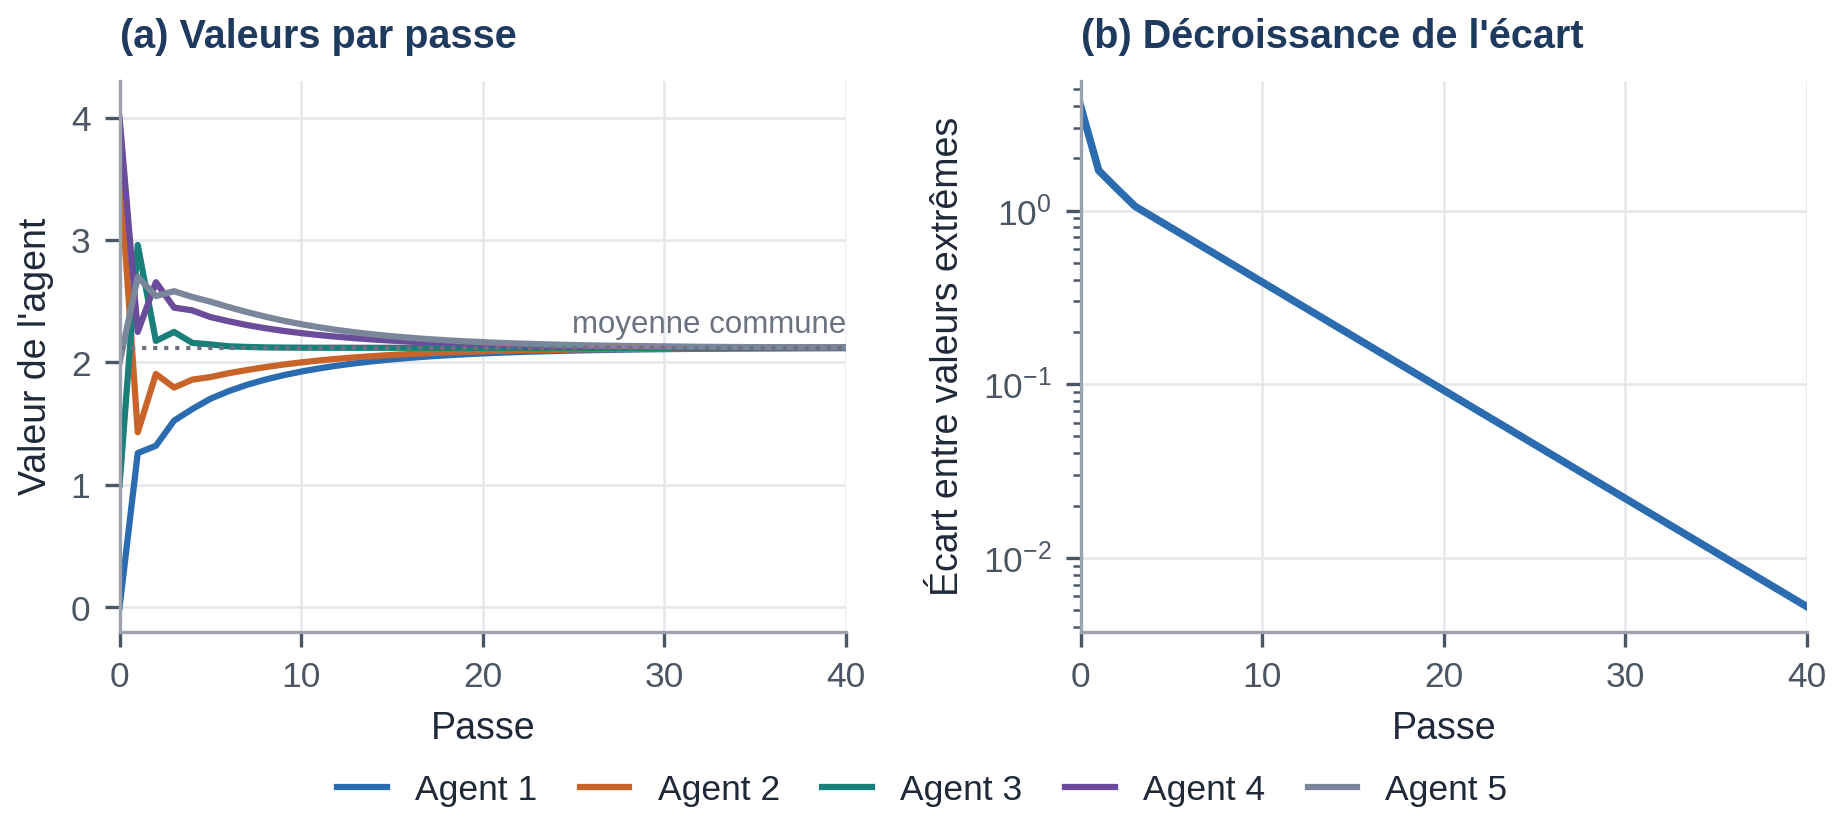
\includegraphics[width=\linewidth,keepaspectratio]{images/consensus_dynamics.png}
  \caption{Consensus sur un graphe linéaire de cinq agents. À gauche, évolution des valeurs à chaque passe ; à droite, décroissance de l'écart entre les valeurs extrêmes sur une échelle logarithmique. Illustration de l'auteur, adaptée des principes de consensus et de l'analyse graph-théorique présentés dans \cite{olfati2004,mesbahi2010}.}
  \label{fig:consensus-convergence}
\end{figure}

Ce cadre diffère du problème étudié dans ce mémoire à plusieurs égards. L'état partagé y est un scalaire ou un vecteur, la mise à jour est linéaire et la tâche est de s'accorder, non de produire une géométrie. Ici, la sortie est une commande de mouvement, la mise à jour est non linéaire et paramétrée, et la cible n'est pas négociée entre robots : elle est fournie par consigne. Le parallèle n'en reste pas moins méthodologiquement utile pour deux raisons. La première est diagnostique : lorsque l'essaim échoue, il faut pouvoir distinguer un échec de la loi de contrôle d'une rupture de connectivité, ce qui impose de surveiller le graphe de communication. La seconde est structurelle : l'agrégation des messages dans le contrôleur proposé est une version apprise d'une opération d'agrégation voisine de celle du consensus, avec la même propriété d'invariance par réordonnancement.

\section{Flocking et comportements locaux}

Le flocking désigne un déplacement collectif dans lequel les agents restent groupés tout en conservant une direction de mouvement cohérente. Dans sa forme classique, il combine trois idées. La cohésion rapproche un agent du centre de ses voisins. La séparation produit une force opposée lorsque deux agents deviennent trop proches. L'alignement rapproche la vitesse d'un agent de la vitesse moyenne observée autour de lui. Ces mécanismes ne nécessitent pas de chef, car chaque robot applique la même règle à partir de son voisinage \cite{reynolds1987}. La Figure~\ref{fig:flocking-rules} décompose visuellement ces trois contributions sur un essaim miniature ; le robot orange, dont on cherche le déplacement, pondère localement les trois flèches selon son propre voisinage.

\begin{figure}[htbp]
  \centering
  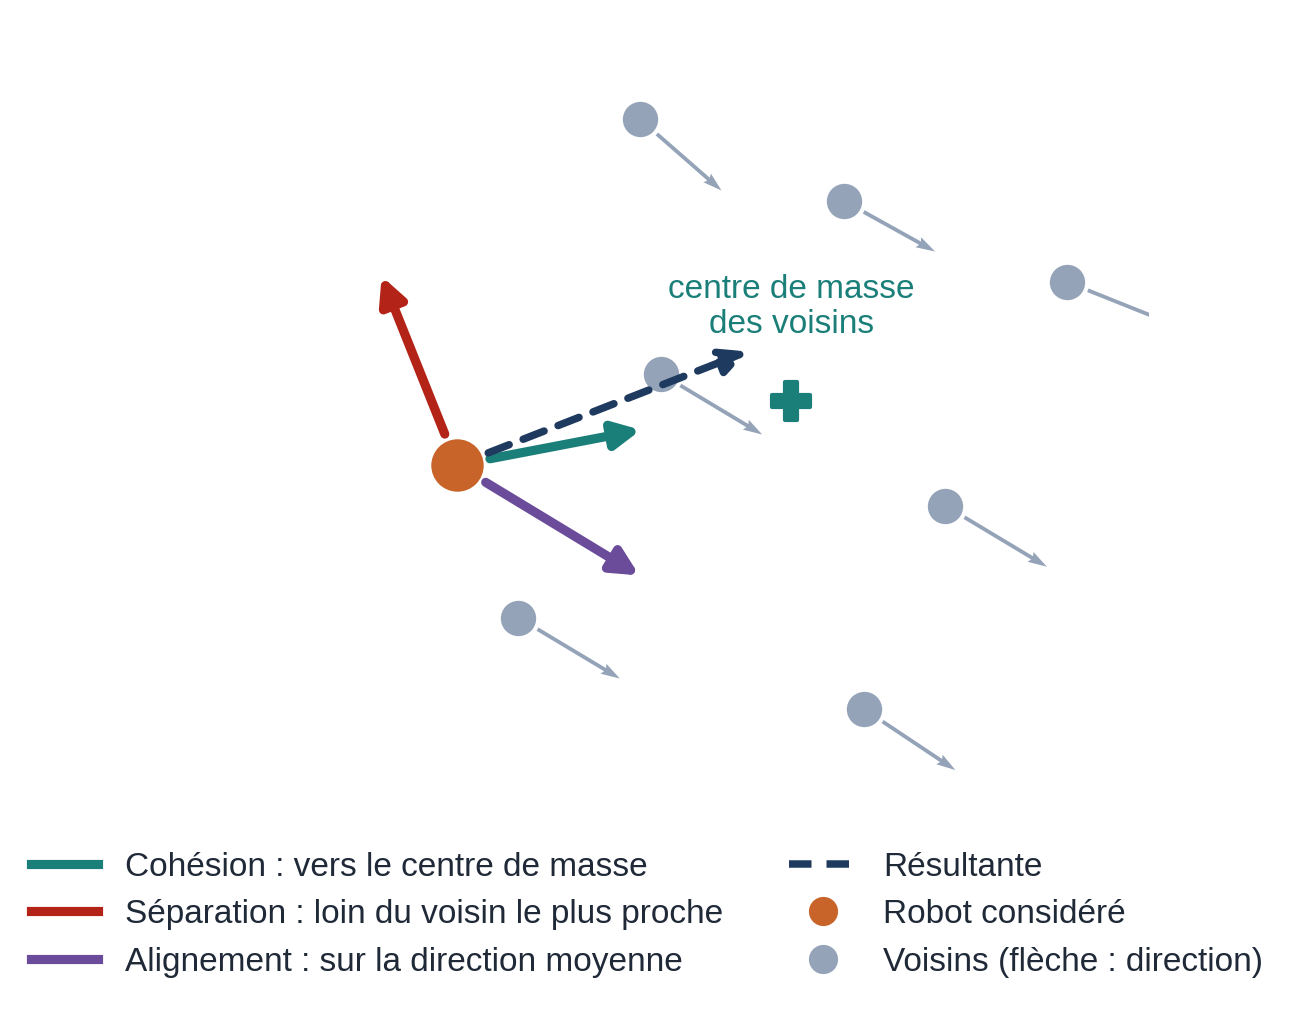
\includegraphics[width=\linewidth,keepaspectratio]{images/flocking_rules.png}
  \caption{Les trois contributions d'une règle de flocking appliquées au robot orange : attraction vers le centre de masse des voisins (cohésion), éloignement du voisin le plus proche (séparation) et alignement sur la direction moyenne du groupe. Illustration de l'auteur, adaptée des règles comportementales de Reynolds \cite{reynolds1987}.}
  \label{fig:flocking-rules}
\end{figure}

Cette famille de règles est une référence utile pour deux raisons. D'abord, elle donne un comportement de base facilement interprétable : si les robots s'accumulent, on peut renforcer la séparation ; s'ils se dispersent, on peut renforcer la cohésion. Ensuite, elle montre que des interactions très simples suffisent à créer un comportement collectif. Dans le prototype, la règle de cohésion-répulsion a joué ce rôle de contrôle : elle a servi à vérifier que le simulateur et le calcul de voisinage produisaient un regroupement avant l'introduction du GNN. Cette vérification appartient au pilote historique, non à une nouvelle expérimentation.

Le flocking ne résout toutefois pas directement la formation de formes. Un essaim peut rester cohérent et se déplacer de manière alignée tout en restant loin du contour demandé. Ajouter une attraction vers une cible est possible, mais il faut alors définir comment chaque robot choisit une zone du contour et comment éviter que tous convergent vers le même endroit. C'est précisément l'espace de décision que l'apprentissage cherche à explorer dans ce mémoire. Le GNN ne remplace pas les idées de cohésion ou de séparation par magie ; il apprend une fonction de décision qui peut utiliser les vitesses, les distances et les messages du voisinage pour réduire la perte définie pendant l'entraînement.

\section{Géométrie de la cible et consigne partagée}

La formation de formes vise à faire converger les positions des robots vers une structure spatiale : une courbe, une formation rigide, une surface ou un nuage de points. Plusieurs représentations sont envisageables. Une cible peut être décrite par une équation analytique, par des positions de référence attribuées aux robots, par une carte, par des points de contour ou par des informations perceptives. Chaque choix modifie la difficulté du problème. Une affectation fixe robot--point fournit une information très forte, mais impose de résoudre l'association et peut limiter l'adaptation aux pannes. À l'inverse, une simple étiquette de forme contient peu de géométrie : elle est facile à partager, mais elle demande au contrôleur d'apprendre comment cette étiquette doit modifier le comportement.

Le présent projet utilise des nuages de points comme représentation de la cible. Cette représentation évite de lier durablement un robot particulier à un point particulier ; la qualité de formation est mesurée par la proximité entre les deux ensembles de points. Elle doit cependant être interprétée correctement. Le nuage cible est une consigne de mission définie avant le déploiement ; son accès n'est pas une communication entre robots. Lorsque la configuration utilise le vecteur vers le point de contour le plus proche, elle suppose une forme de carte ou de requête géométrique locale. Cette hypothèse facilite la formation de contours complexes, mais elle ne doit pas être confondue avec une perception autonome de la forme dans un environnement réel.

\section{Réseaux de neurones sur graphes et passage de messages}

Un essaim à voisinage local se modélise naturellement par un graphe dynamique $\mathcal{G}^t=(\mathcal{V},\mathcal{E}^t)$. Chaque robot est un nœud ; une arête relie deux robots lorsqu'ils peuvent échanger des informations au pas de temps $t$. Les réseaux de neurones sur graphes étendent les réseaux neuronaux à ce type de données relationnelles. Dans le cadre du passage de messages, un nœud produit ou reçoit des messages calculés à partir des états des nœuds reliés et des attributs d'arête, puis agrège ces messages avant de mettre à jour sa représentation \cite{gilmer2017}. Le cadre plus général des \emph{graph networks} formalise de la même façon les mises à jour de nœuds, d'arêtes et, éventuellement, d'attributs globaux \cite{battaglia2018}.

Deux propriétés rendent ce formalisme particulièrement adapté au contrôle d'essaim. D'abord, les paramètres sont partagés : la même fonction de message et la même fonction de décision peuvent être utilisées pour chaque robot. Ensuite, une agrégation par somme, moyenne ou maximum est invariante à l'ordre des voisins. Un robot peut donc recevoir un nombre différent de messages au cours du temps sans qu'il soit nécessaire de modifier la taille de l'entrée du réseau. Ces propriétés ne garantissent pas à elles seules une bonne généralisation, mais elles introduisent un biais inductif cohérent avec le caractère relationnel et variable d'un essaim.

\subsection{Fonctions d'activation}

Une succession de transformations affines sans activation reste une transformation affine. Les fonctions d'activation introduisent la non-linéarité nécessaire pour représenter des réponses différentes selon l'observation et les messages reçus. Dans le modèle actuel, ReLU conserve les entrées positives et annule les entrées négatives : $\mathrm{ReLU}(z)=\max(0,z)$. Sa pente vaut un du côté positif et zéro du côté négatif ; la fonction n'est pas dérivable en zéro. Cette propriété ne garantit pas une optimisation sans difficulté, et une unité inactive peut recevoir un gradient nul.

La tangente hyperbolique joue un autre rôle : elle ramène chaque composante dans l'intervalle $(-1,1)$. Le décodeur l'emploie avant une limitation de la norme totale de la commande. Elle ne doit donc pas être confondue avec ReLU ni présentée comme suffisante, seule, pour garantir la borne de vitesse en deux dimensions. La Figure~\ref{fig:activation-functions} distingue ces deux fonctions par leurs courbes exactes, sans exemple d'apprentissage.

\begin{figure}[htbp]
  \centering
  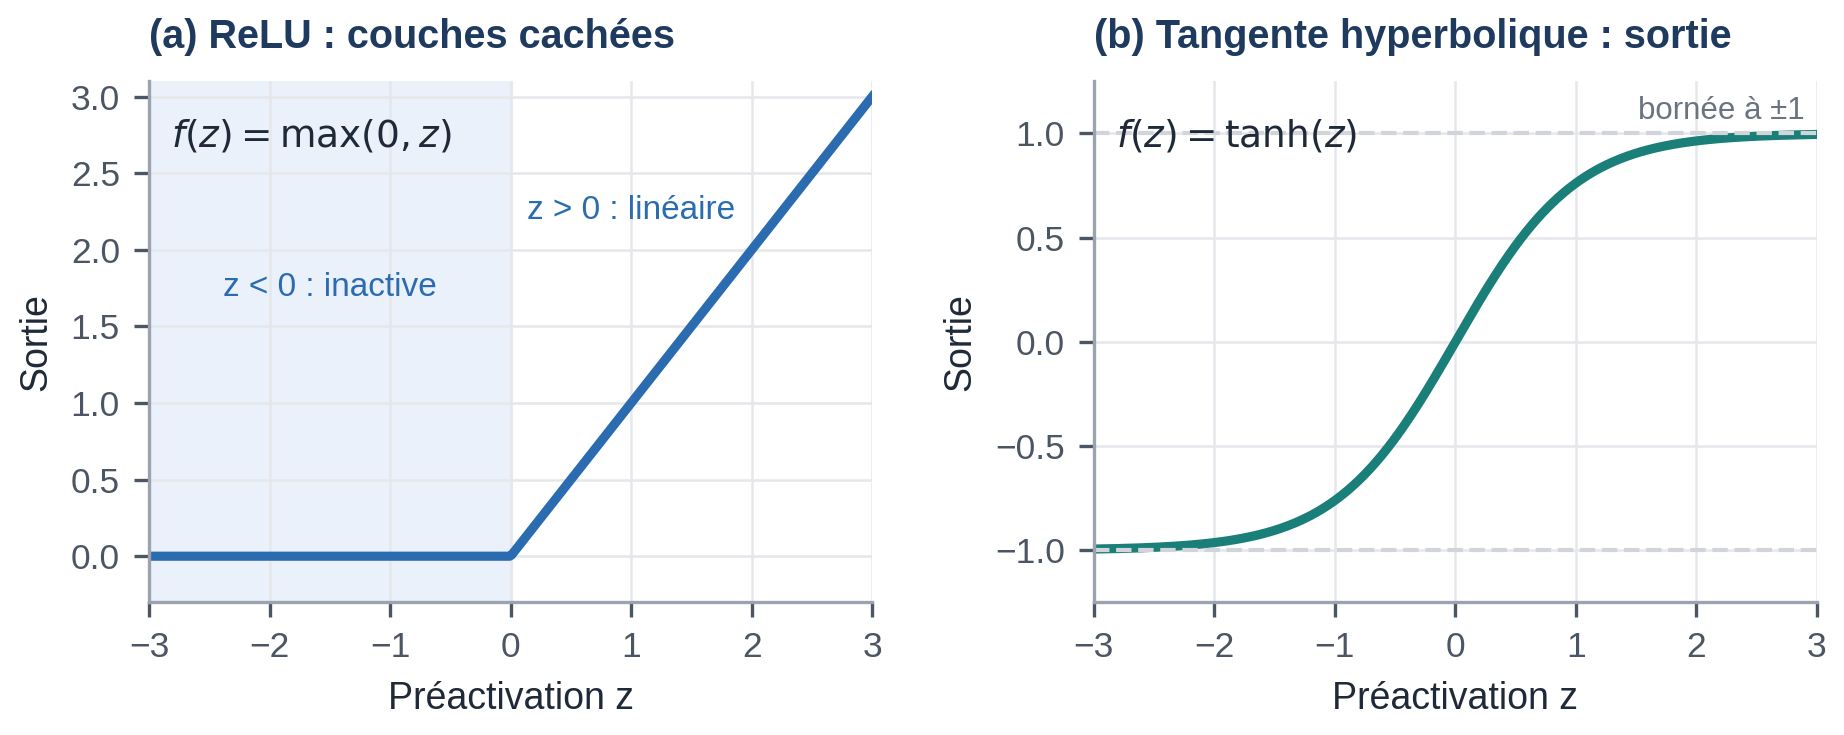
\includegraphics[width=\linewidth,height=.65\textheight,keepaspectratio]{images/activation_functions.png}
  \caption[Fonctions ReLU et tangente hyperbolique]{Courbes mathématiques exactes des fonctions ReLU et tangente hyperbolique. ReLU intervient dans les représentations internes ; la tangente hyperbolique intervient à la sortie avant une projection limitant la norme. Illustration originale des fonctions présentes dans le modèle, non issue d'une expérience.}
  \label{fig:activation-functions}
\end{figure}

\subsection{Agrégation locale des messages}

Dans le contrôleur implémenté, l'agrégation est une moyenne. Chaque voisin $j$ envoie d'abord un message $m_{ij}$ calculé à partir de son état, de l'état du robot $i$ et de leur géométrie relative. Le robot $i$ calcule ensuite la moyenne de ces messages sur son voisinage $\mathcal{N}(i)$. La division par le nombre de voisins retire le facteur multiplicatif du degré présent dans une somme brute. La norme de cette somme ne croît toutefois pas nécessairement avec le degré, car les messages peuvent se compenser. La moyenne ne garantit donc ni une distribution stable des messages ni la qualité de formation. Lorsqu'un robot n'a aucun voisin, l'agrégat est remplacé par un vecteur nul, puis le réseau produit tout de même une commande à partir de son état propre et de la consigne ; cela ne garantit pas sa pertinence ni sa sécurité. La Figure~\ref{fig:aggregation-mean} illustre ce principe d'agrégation localement appliqué par chaque robot.

\begin{figure}[htbp]
  \centering
  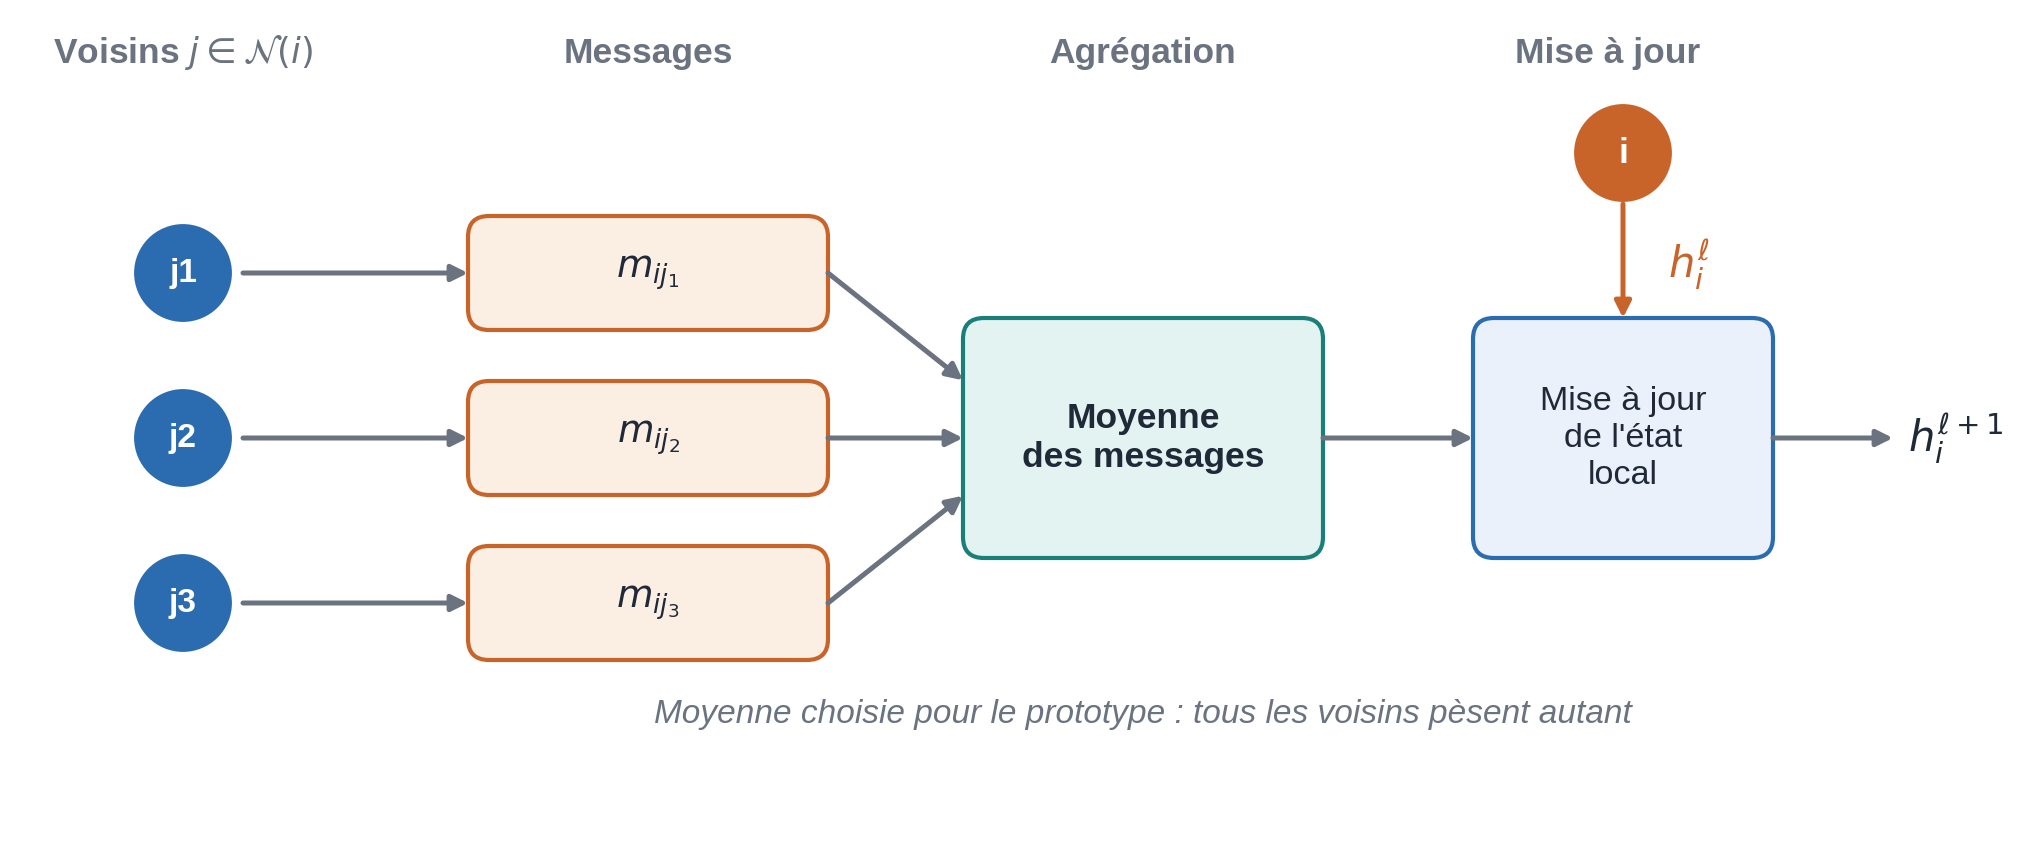
\includegraphics[width=\linewidth,keepaspectratio]{images/message_aggregation.png}
  \caption{Principe d'agrégation employé dans le contrôleur. Les messages individuels sont calculés pour chaque voisin, puis leur moyenne est utilisée pour mettre à jour l'état local du robot. Illustration de l'auteur, adaptée du cadre de passage de messages \cite{gilmer2017,battaglia2018} pour représenter le choix de moyenne du prototype.}
  \label{fig:aggregation-mean}
\end{figure}

\subsection{Profondeur et portée informationnelle}

Le passage de messages possède également une limite structurelle : avec $L$ tours d'échange, l'état d'un robot ne peut intégrer directement que les informations disponibles dans son voisinage à au plus $L$ sauts, pour la topologie considérée. La Figure~\ref{fig:message-depth} rend cette portée concrète : le robot $i$ au centre reçoit, après un tour, les informations de son anneau immédiat ; après deux tours, celles de l'anneau suivant ; au-delà, l'information est structurellement absente de son état. Augmenter $L$ peut étendre la portée informationnelle, mais augmente aussi le coût de calcul et peut rendre l'apprentissage plus difficile. Un GNN ne transforme donc pas un système local en contrôleur centralisé : il fournit une manière paramétrable d'exploiter des communications restreintes.

\begin{figure}[htbp]
  \centering
  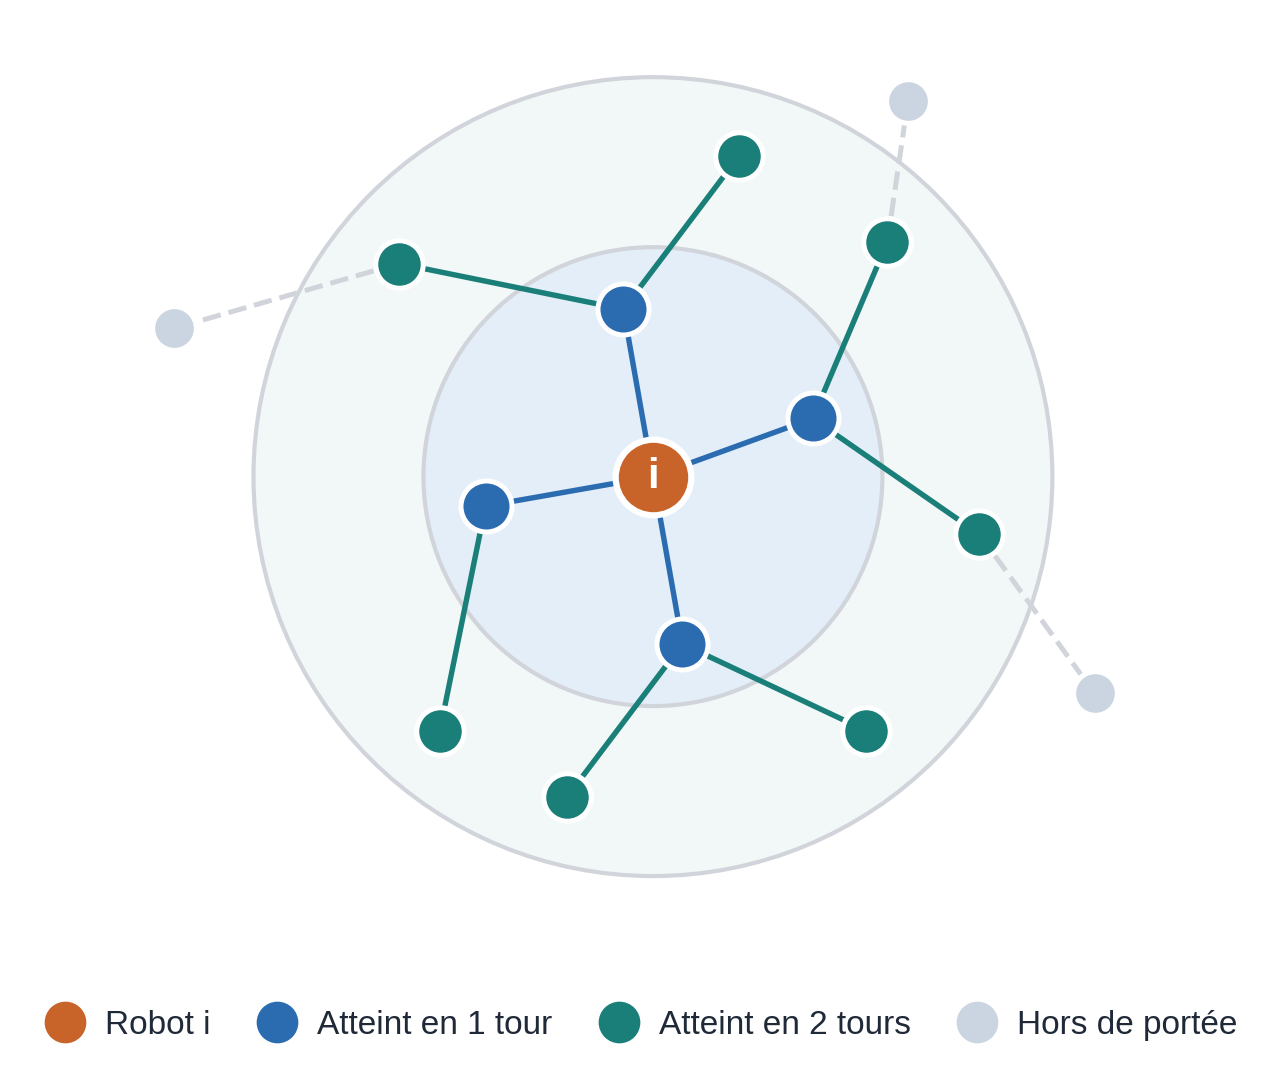
\includegraphics[width=\linewidth,keepaspectratio]{images/information_reach.png}
  \caption{Portée de l'information selon le nombre de tours de messages. Chaque anneau correspond à un saut supplémentaire dans le graphe de communication ; le prototype des résultats pilotes historiques utilise deux tours. Illustration de l'auteur, adaptée du principe de passage de messages \cite{gilmer2017,battaglia2018}.}
  \label{fig:message-depth}
\end{figure}

\subsection{Induction et changement d'échelle}

La possibilité d'appliquer un même modèle à une taille d'essaim différente est souvent associée au caractère inductif des architectures de graphe. Dans GraphSAGE, Hamilton, Ying et Leskovec apprennent une fonction qui agrège les attributs d'un voisinage local au lieu d'apprendre un vecteur propre à chaque nœud \cite{hamilton2017}. Le problème traité dans cet article est différent de la robotique, mais le principe est utile ici : une politique ne doit pas dépendre de l'identifiant d'un robot ni d'une liste d'entrée de longueur fixe.

Cette propriété ne doit pas être présentée comme une garantie de performance. Lorsque le nombre de robots augmente, la densité locale, la connectivité et le nombre moyen de voisins peuvent aussi changer. Une politique peut donc être techniquement exécutable avec cent robots tout en produisant une formation moins régulière que pour vingt robots. Le passage à l'échelle doit être mesuré, avec une cible et des conditions initiales adaptées, plutôt que supposé à partir de l'architecture.

\section{Conclusion partielle}

Ce chapitre a défini les concepts de robotique en essaim, d'auto-organisation, de consensus et de flocking, puis précisé les représentations de cible et le fonctionnement local du passage de messages sur graphe. La connectivité, l'invariance à l'ordre des voisins et le partage des paramètres fournissent des outils pour concevoir et analyser une politique décentralisée, sans garantir sa convergence vers une forme, sa robustesse ni son passage à l'échelle. Le chapitre suivant présente l'état de l'art : il compare les méthodes traditionnelles et avancées, examine quelques études connexes et situe le prototype au regard de leurs hypothèses et de leurs limites.
